\chapter{Ergebnisse der Literaturrecherche}

\section{Chronologische Entwicklung der Lehr- und Lernmaschinen}

\subsection{Mechanische Maschinen}

Die Entwicklung didaktischer Simulatoren lässt sich über mehrere Jahrhunderte hinweg nachzeichnen. Erste Vorläufer finden sich bereits 1588, als Agostino Remelli ein sogenanntes \textit{Leserad} konzipierte, das die parallele Nutzung mehrerer Bücher erleichtern sollte und somit als frühe mechanische Lernhilfe gelten kann.\parencite{cayetano_geschichte_2022}

Ein bedeutender Meilenstein in der Entwicklung früher Lernmaschinen wurde im Jahr 1866 durch das Patent von Halycon Skinner gesetzt. Er konstruierte ein Gerät, bei dem nach der visuellen Darstellung eines Bildes auf einem Kasten die korrekte Bezeichnung über eine Schreibmaschinentastatur eingegeben werden musste. Die Maschine erwies sich jedoch als äußerst fehleranfällig: Falsche Begriffe wurden bei korrekter Orthographie als richtig gewertet, was die Zuverlässigkeit des Systems stark einschränkte. Im Jahr 1911 griff Herbert Aiken Skinners Konzept auf und entwickelte eine verbesserte Version, die er als „Buchstabiermaschine“ präsentierte. Diese Lernvorrichtung basierte auf einem mechanischen Rahmen, in den mit Buchstaben beschriftete Karten eingesetzt wurden. Die puzzleartige Konstruktion erlaubte das Ausprobieren verschiedener Kombinationen, wobei ausschließlich die korrekte Lösung zum Erfolg führte und das „Puzzle“ vervollständigte. Bis 1936 wurden rund 700 Patente für derartige Übungsmaschinen angemeldet. Das grundsätzliche Lernkonzept hinter diesen Maschinen ist das \textit{law of effect} des amerikanischen Psychologen Edward L. Thorndike.\parencite[S.~3]{niegemann_kompendium_2008}

Bereits 1928 stellte \textbf{Sidney Leavitt Pressey} eine „Maschine für Intelligenztests“ vor, die zu den einflussreichsten Vorläufern späterer Lehrmaschinen zählt. Sie arbeitete mit Multiple-Choice-Aufgaben, wobei die Lernenden ihre Antworten über nummerierte Tasten eingaben. Ein eingebauter Zähler registrierte die Anzahl richtiger Lösungen. Bemerkenswert ist, dass Pressey darüber hinaus -- in Anlehnung an das zeitgleich entwickelte „law of effect“ -- einen Belohnungsmechanismus integrierte: Bei einer korrekten Antwort gab die Maschine eine Süßigkeit aus. Damit machte Pressey deutlich, dass psychologische Faktoren wie Motivation und Verstärkung zentrale Elemente bei der Gestaltung von Lern- und Lehrmaschinen sein können.\parencite[S.~705]{benjamin_history_1988}\parencite[S.~969f]{skinner_teaching_1958}

In den 1950er Jahren erhielten die von \textbf{Burrhus F. Skinner} und \textbf{James G. Holland} entwickelten Lehrmaschinen zunehmende Aufmerksamkeit. Diese „Skinner-Holland’schen Maschinen“ beruhten explizit auf der behavioristischen Lerntheorie und folgten dem Prinzip des programmierten Lernens: Der Stoff wurde in kleine Einheiten (\textit{Frames}) zerlegt, auf die jeweils Fragen folgten. Lernende konnten ihre Eingabe direkt mit der richtigen Lösung vergleichen und erhielten so unmittelbares Feedback.\parencite[S.~970--977]{skinner_teaching_1958} Bereits hier lassen sich die zentralen Prinzipien des programmierten Unterrichts erkennen: die Strukturierung des Lernstoffs in kleine Schritte, die Anpassung an das individuelle Lerntempo, die aktive Beteiligung durch Antworten sowie die sofortige Rückmeldung.\parencite[S.~1971]{bruillard_teaching_2020} Diese didaktischen Grundsätze wurden in den 1960er Jahren auf den Computer übertragen und bildeten die Basis für die Entwicklung der computergestützten Instruktion.

Im Gegensatz zu den linearen Lehrprogrammen entwickelte \textbf{Norman Crowder} im Jahr 1959 das Konzept der sogenannten „verzweigten Lernprogramme“, die eine erste Form der Individualisierung im Lehr-Lernprozess ermöglichten. Diese Programme reagierten adaptiv auf die Fehler der Lernenden, indem sie unterschiedliche Lernpfade eröffneten. Charakteristisch für Crowders Ansatz sind umfangreichere Frames, die jeweils durch eine Multiple-Choice-Frage abgeschlossen werden. Bei Auswahl einer falschen Antwort erhielt der Lernende eine spezifische Rückmeldung, die auf die Art des Fehlers abgestimmt war. Anschließend führte das Programm entlang einer fehlerabhängigen Sequenz weiter, wobei zuvor behandelte Inhalte bei Bedarf erneut präsentiert wurden, sofern ein Verständnisdefizit vermutet wurde.\parencite[S.~252--254]{crowder_differences_1963}\parencite[S.~9]{schonfeld_computerbasiertes_2006} Crowders Ansatz gilt damit als wichtiger Schritt hin zu adaptiven Lernsystemen, die später in den 1960er Jahren mit dem Aufkommen computergestützter Instruktion (CAI) technisch umgesetzt werden konnten.

\subsection{Computergestützte Instruktion}

\sh{Entwicklungen in den USA}
 Ab den 1960er Jahren fanden computergestützten Instruktion (CAI – Computer Assisted Instruction) zunächst weite Verbreitung, verloren jedoch Mitte des Jahrzehnts an öffentlicher Aufmerksamkeit. Neue Impulse gingen von großangelegten US-Projekten aus, die 1971 durch die National Science Foundation initiiert wurden. Dazu zählten \textit{PLATO} (Programmed Logic for Automatic Teaching Operation) und \textit{TICCIT} (Time-shared Interactive Computer Controlled Information Television), die erstmals computerbasierte Instruktion in großem Maßstab demonstrierten.\parencite[S.~7]{niegemann_kompendium_2008}\parencite[S.~69]{oshea_lernen_1986}

\textit{TICCIT} ermöglichte den Lernenden eine individuelle Steuerung ihres Lernprozesses, insbesondere in den Fächern Mathematik und Englischaufsatz. Während bei vollständiger Nutzung gute Lernergebnisse erzielt wurden, war die Abbruchquote deutlich höher als im Präsenzunterricht. Als Ursachen gelten mangelnde Selbstorganisation der Lernenden sowie die geringe Akzeptanz durch Lehrende, was letztlich zum Scheitern des Projekts beitrug. Dennoch gilt TICCIT als technologisch bedeutsamer Fortschritt.\parencite[S.~13]{schonfeld_computerbasiertes_2006}\parencite[S.~71]{oshea_lernen_1986}

\textit{PLATO} bot im Vergleich dazu eine weiterentwickelte Form computerunterstützter Instruktion, die vor allem durch interaktive Simulationen am Bildschirm überzeugte. Zwar waren die Lernergebnisse ähnlich wie bei TICCIT, jedoch war die Abbruchquote geringer, und viele Lernende nutzten das System freiwillig über die Kurszeiten hinaus. PLATO gilt daher als besonders motivationsförderndes Lernsystem mit hoher Nutzerbindung.\parencite[S.~14]{schonfeld_computerbasiertes_2006}\parencite[S.~75f]{oshea_lernen_1986}

\sh{Entwicklungen in Deutschland und Europa}
Parallel zu den großangelegten US-Projekten entstanden in Deutschland ab 1964 verschiedene Lehrmaschinen, darunter der \textit{Robbimat 0}, der \textit{Geromat III} und der \textit{Bakkalaureus}, die vor allem für die Gruppenschulung eingesetzt wurden. Weitere Forschungsinitiativen bildeten sich mit dem Bildungstechnologischen Zentrum in Wiesbaden sowie dem „Forschungs- und Entwicklungszentrum für objektivierte Lehr- und Lernverfahren“ (FEoLL) in Paderborn. In Berlin wurde zudem das Projekt \textit{ALCU} (Algorithmierung von Lehrprogrammen für computergesteuerten Unterricht) erprobt, das die systematische Erstellung von Lehrprogrammen für den computergestützten Unterricht zum Ziel hatte.\parencite[S.~10]{niegemann_kompendium_2008}\parencite[S.~11]{schonfeld_computerbasiertes_2006}

In den frühen 1970er Jahren entstanden an der Universität Freiburg Programme wie \textit{PFLABE}, das Biologiestudierenden Wissen als Ersatz für Praktika vermitteln sollte, sowie \textit{ZOPRAM}, das darauf abzielte, Vorwissensunterschiede zwischen Studierenden auszugleichen. Die Begleituntersuchungen zeigten, dass der Lernerfolg von \textit{PFLABE}-Nutzenden nicht über dem der Vergleichsgruppe im Praktikum lag, jedoch der Zeitaufwand für das Lernen mit dem Programm deutlich geringer war. Gleichzeitig wurden auch Simulationsprogramme entwickelt, die praxisnahes Lernen in experimentellen Szenarien unterstützen sollten.\parencite[S.~11]{niegemann_kompendium_2008}

Nach einer Phase des Rückgangs in den späten 1970er und frühen 1980er Jahren erlebte das computergestützte Lernen Mitte der 1980er Jahre eine Renaissance, insbesondere durch methodisch anspruchsvollere Programme wie \textit{KAVIS}/\textit{KAVIS II} für den Biologieunterricht. Ab Mitte der 1990er Jahre gewann computergestütztes Lernen durch die zunehmende Verfügbarkeit von Personal Computern und den Aufschwung des World Wide Webs (siehe dazu Abb.~\ref{fig:rechner_internet}und Abb.~\ref{fig:internetnutzer} ) erneut erheblich an Bedeutung und führte schließlich zur Etablierung des Begriffs „E-Learning“.\parencite[S.~11]{niegemann_kompendium_2008}

\begin{figure}[h!]
    \centering
    \begin{subfigure}[b]{0.48\textwidth}
        \centering
        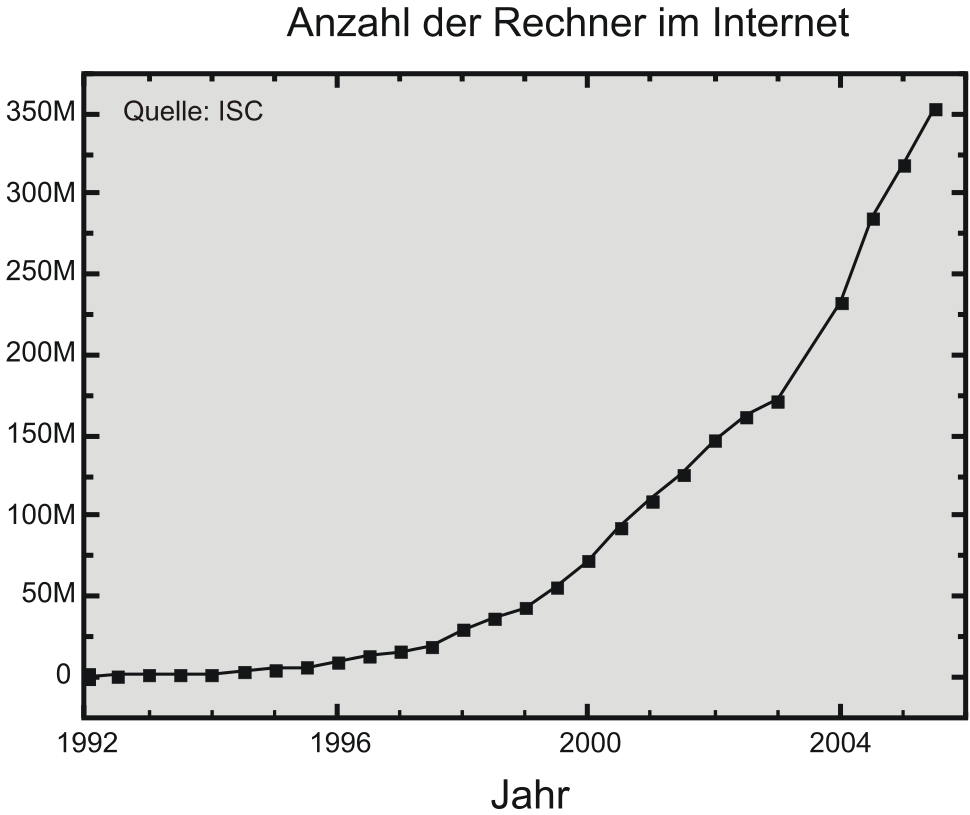
\includegraphics[width=\textwidth]{img/Anzahl_Rechner_im_Internet-2004.png}
        \caption{Anzahl der Rechner im Internet}
        \label{fig:rechner_internet}
		\cite{internet_systems_consortium_internet_2005}
    \end{subfigure}
    \hfill
    \begin{subfigure}[b]{0.48\textwidth}
        \centering
        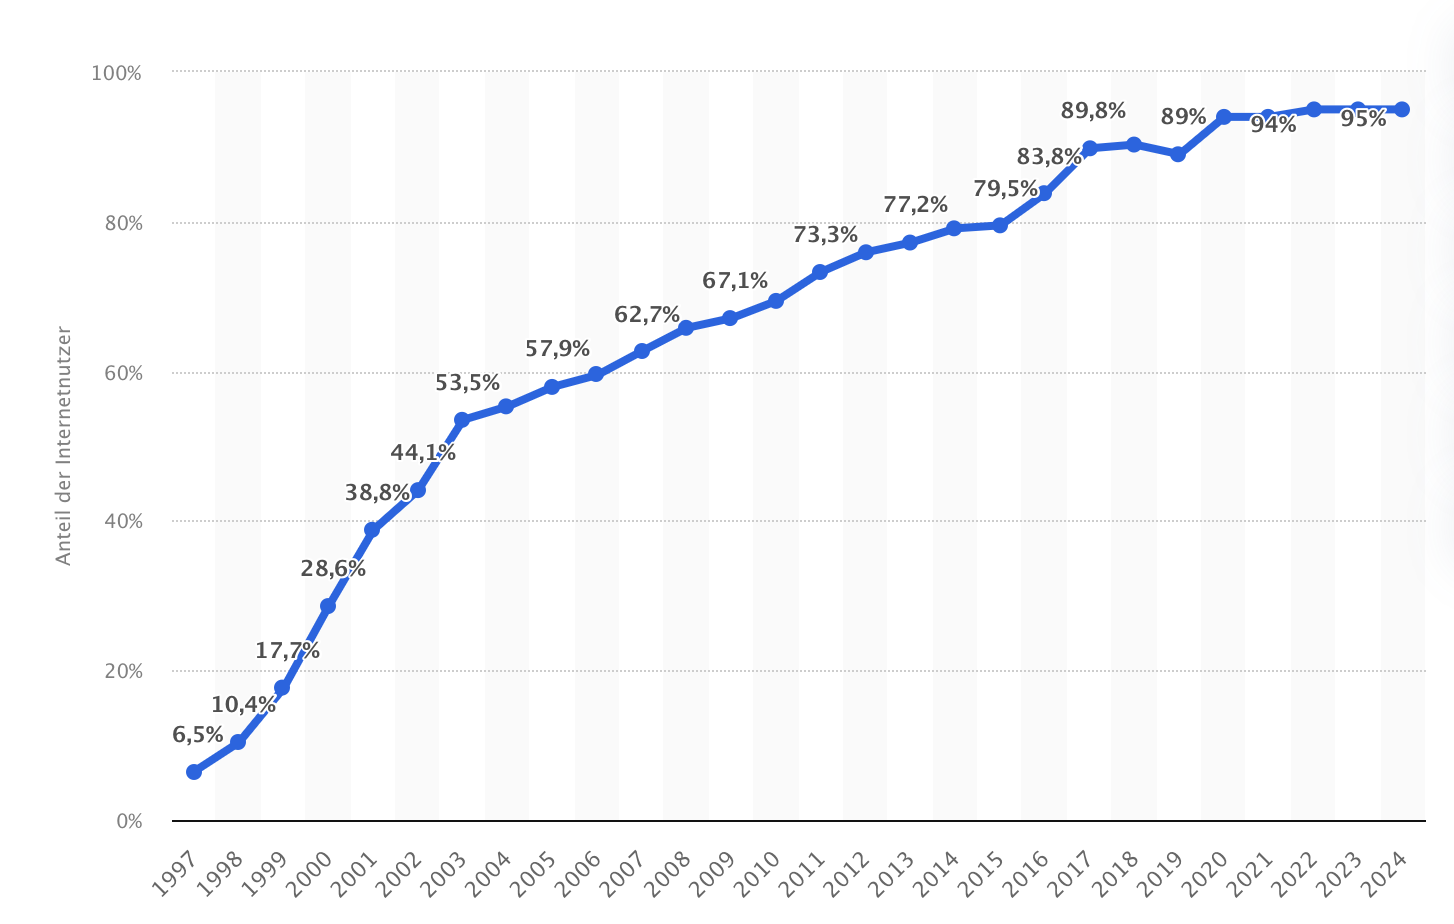
\includegraphics[width=\textwidth]{img/Anzahl_Internetnutzer-2024.png}
        \caption{Internetnutzer in DE 1997 bis 2024}
        \label{fig:internetnutzer}
		\cite{statista_anteil_2024}
    \end{subfigure}
    \caption{Entwicklung des World Wide Webs}
    \label{fig:www}
\end{figure}

\subsection{Neuere Entwicklungen}

Mit der Initiative „Schulen ans Netz“ \cite{schulen_ans_netz_ev_schulen_nodate} wurde im Jahr 2001 die flächendeckende Internetanbindung deutscher Schulen erreicht.\cite{kopcke_internet_2016} In den 2000er Jahren entstanden zahlreiche vom Bundesministerium für Bildung und Forschung (BMBF) geförderte Projekte, die sich speziell mit der Visualisierung und Simulation in der Informatik-Didaktik befassten. Dazu zählen unter anderem \textit{SIMBA} (Schlüsselkonzepte der Informatik in multimedialen Bausteinen)\footnote{Das BMBF-Verbundprojekt SIMBA und darin das Teilprojekt Rechnernetze basieren auf netzbasiertem Lernmaterial wie Hypertexten, Grafiken und Animationen.\parencite[S.~75]{magenheim_blended_2003}}, \textit{MuSofT} (Multimedia in der Softwaretechnik)\footnote{Ziel des MuSofT-Projekts war es, für die Software-Engineering-Ausbildung multimediale Materialien bereitzustellen und ein Konzept für Blended Learning zu entwickeln.\parencite[S.~73]{magenheim_blended_2003}}, \textit{RaVi} (Rechnerarchitektur-Visualisierung)\footnote{Das RaVi-Projekt machte dynamische Abläufe in Rechnersystemen anschaulich und berücksichtigte dabei gezielt frauenspezifische Lerninteressen.\parencite[S.~20]{marwedel_interaktive_2003}} sowie die Wissenswerkstatt Rechensysteme (\textit{WWR})\footnote{WWR ist ein Baukastensystem aus multimedialen, skalier- und rekombinierbaren Lehr- und Lernmodulen.\parencite[S.~1]{kornelsen_inhalte_2004}}. Alle diese Projekte verfolgten das Ziel, komplexe Vorgänge in Rechnersystemen durch interaktive und multimediale Simulationen für Lernende erfahrbar zu machen.

 1. Web 2.0 und die Etablierung von Lernplattformen (LMS):
       * Nach der "Schulen ans Netz"-Initiative wurde die Software-Infrastruktur entscheidend. Die Verbreitung von Learning Management Systems (LMS) wie Moodle oder ILIAS (im deutschsprachigen
         Raum sehr verbreitet) hat die Bereitstellung und Organisation von digitalen Lerninhalten standardisiert. Diese Plattformen wurden zum zentralen Ort für viele der von dir genannten
         Simulationen.

   2. MOOCs (Massive Open Online Courses) – ab ca. 2012:
       * Die Entstehung von Plattformen wie Coursera, Udacity und edX hat die Hochschulbildung revolutioniert. Sie haben gezeigt, dass hochwertige Kurse (inkl. Simulationen und interaktiven
         Aufgaben) für eine riesige Anzahl von Lernenden global zugänglich gemacht werden können.

   3. Mobile Learning (M-Learning):
       * Mit der flächendeckenden Verbreitung von Smartphones und Tablets verlagerte sich das Lernen vom reinen Desktop-PC hin zu mobilen Endgeräten. Didaktische Konzepte mussten angepasst
         werden, um "Lernen jederzeit und überall" zu ermöglichen (z.B. durch Apps, responsive Webseiten).

   4. Gamification:
       * Dies ist eine direkte Weiterentwicklung der von Pressey eingeführten Belohnungsmechanismen. Die Anwendung von Spielmechaniken (Punkte, Abzeichen, Ranglisten) in Lernkontexten wurde zu
         einem wichtigen Trend, um die Motivation zu steigern. Viele moderne Simulatoren nutzen diese Elemente.

   5. Immersive Lernumgebungen (VR/AR):
       * Ein riesiger Sprung für Simulatoren. Mit Virtual Reality (VR) und Augmented Reality (AR) können Lernende vollständig in eine simulierte Umgebung eintauchen. Anwendungsfälle sind z.B.
         die Pilotenausbildung, medizinische Operationstrainings oder das Üben an virtuellen Maschinen in der Technik. Dies ist eine der aktuellsten Formen des didaktischen Simulators.

   6. Künstliche Intelligenz (KI) in der Bildung:
       * Dies ist der aktuellste und vielleicht wichtigste Trend, der direkt an Crowders adaptive Systeme anknüpft:
           * Intelligente Tutorielle Systeme (ITS): Systeme, die mit KI-Methoden das Wissen und die Fähigkeiten der Lernenden modellieren und hochgradig personalisierte Lernpfade und Feedbacks
             anbieten.
           * Learning Analytics: Die Analyse von Lerndaten, um den Lernprozess zu verstehen, vorherzusagen und zu optimieren.
           * Generative KI (z.B. LLMs): Neueste Modelle können als Dialogpartner, Tutoren oder sogar zur Erstellung von Lerninhalten und einfachen Simulationen dienen.


\TODO{Was sind aktuelle Trends?}
\TODO{Was kann man für Zukunft extrapolieren?}

\section{Überblick anhand von Themen}

\section{Überblick anhand von Simulatortypen}
